\documentclass[a4j, 9pt]{ltjsarticle}

\usepackage{multicol}
\usepackage{amsmath, amssymb, amsfonts} %数学系全般のパッケージ
\usepackage{tikz}
\usetikzlibrary{patterns}%斜線塗りを可能にする
\usepackage{mhchem} %化学用パッケージ
\usepackage{pxrubrica} %ルビを振れるようにする\rubyを追加するパッケージ
\usetikzlibrary{calc}

%label属性のついたものの背景色を白で四角系で塗りつぶす
\tikzset{set label/.style={fill=white,rectangle,inner sep=1}}

%定義記号
\def\ldef{\coloneqq}
\def\define{\stackrel{\mathrm{def}}{=}}
\def\defineProposition{\stackrel{\mathrm{def}}{\Longleftrightarrow}}

%ディスプレイスタイル
\def\ds{\displaystyle}

\setlength{\columnsep}{5mm}
\columnseprule=0.2mm

%multicols上でtableの代わりにfigurehere, tablehereを使う
\makeatletter
\newenvironment{tablehere}
  {\def\@captype{table}}
  {}
\newenvironment{figurehere}
  {\def\@captype{figure}}
  {}
\makeatother

\begin{document}

% 目次の出力
\tableofcontents
\clearpage

\part{基礎の確認}

  \section{集合論}
    数学でモデルを扱うとき集合論的に思考すると上手にそのモデルを扱うことができる。これは数学の問題を解く場合も同様である。では集合論とは何か、概要を確認しておこう。
    \begin{multicols}{2} %*を用いれば真ん中の直線を最初から最大にできる

      \subsection{集合の定義}
        集合とはその名の通り、いくつかのものをひとまとめにして考えた「ものの集まりのこと」である。
        特に集合論では「もの」のことを要素という。\par
        またある集合$\ds A$は他の集合$\ds B$と共通部分を持ったり、はたまたその集合$\ds A$自体が他の集合$\ds B$の一部分となるケースも考えられる。
        そのような場合順に「$\ds AとB$の共通部分」、「$\ds AはBの$部分集合」という。

        \begin{tikzpicture}[auto]
        
          %Ven diagram1
          \def \circleRadius{1}
          \def \leftCirclePoint{(0, 0)}
          \def \rightCirclePoint{(1, 0)}
          \def \centerPointOfShareArea{(0.5, 0)}
          \def \leftCircleNamePoint{(0, 1)}
          \def \rightCircleNamePoint{(1, 1)}

          %Ven diagram2
          \def \circleARadius{0.7}
          \def \circleBRadius{1}
          \def \circleAPoint{(4, -0.2)}
          \def \circleBPoint{(4, 0)}
          \def \circleANamePoint{(4, \circleARadius-0.2)}
          \def \circleBNamePoint{(4, \circleBRadius)}

          \scope
            %Xのベン図
            \clip \leftCirclePoint circle (\circleRadius);
            \fill [fill=white] \rightCirclePoint circle (\circleRadius);
          \endscope

          \scope
            %Yのベン図
            \clip \rightCirclePoint circle (\circleRadius);
            \fill [pattern=north west lines] \leftCirclePoint circle (\circleRadius);
          \endscope

          \draw \leftCirclePoint circle (\circleRadius);
          \draw \rightCirclePoint circle (\circleRadius);
          \node[set label, text=black] (A) at \leftCircleNamePoint {$\ds A$};
          \node[set label, text=black] (B) at \rightCircleNamePoint {$\ds B$};

          %共通部分ラベル
          \draw[semithick, -, stealth] \centerPointOfShareArea--(0.5, -1.5);
          \draw[semithick, -, stealth] (0.5, -1.5)--(-1, -1.5);
          \node[set label, text=black] (CAP) at (-1, -1.5) {$\ds AとBの共通部分$};


          \fill[pattern=north west lines] \circleAPoint circle (\circleARadius);
          \draw                           \circleAPoint circle (\circleARadius);
          \draw                           \circleBPoint circle (\circleBRadius);
          \node[set label, text=black] (A') at \circleANamePoint {$\ds A$};
          \node[set label, text=black] (B') at \circleBNamePoint {$\ds B$};

        \end{tikzpicture}

        \subsubsection{集合の例}
          例として「原子」という集合を考えてみよう。(ここでいう原子は化学の原子を指すものとする)\par
          原子には様々な種類があり、例えば水素原子\ce{_{1}H}や酸素原子\ce{_{8}O}などがある。
          このとき\ce{_{1}H}や\ce{_{8}O}は原子集合の要素であるといえる。\par
          またさらに水素元素\ce{H}や酸素元素\ce{O}はそれぞれ水素原子\ce{_{1}H}の全同位体を含んだ集合、酸素原子\ce{_{8}O}の全同位体を含んだ集合ゆえ原子集合の部分集合である。

      \subsection{集合論の記号}
        ここまでは言葉を用いて集合について少し語ってきた。しかしいちいち言葉で説明するのは少々面倒であり、しかも読みづらい。そこで記号を導入してみよう。

        \subsubsection{基本的な記法}
          例えば$\ds A$という集合を自然数$\ds 1 \thicksim 5$を要素に持つ集合として定義したい場合$\ds A \define \{ 1, 2, 3, 4, 5 \}$と書く。
          つまり要素を$\ds \{\}$で囲むことでそれらを要素に持つという意味を表すのである。
          この記法を\ruby{外延的記法}{がい|えん|てき|き|ほう}という。\par
          ついでこの場合$\ds 1$は$\ds A$の要素であるから、これを$\ds 1 \in A$と書く。\par
          
          %強制的に改段
          %\columnbreak
          
          また、同じ意味の定義で\par
          $\ds A \define \{ n \in \mathbb{N} \mid 1 \leq n \leq 5 \}$と表すこともできる。
          この場合は具体的に要素を書き出すことをせずに、\par
          $\ds \{ n \in ($母体となる集合$\ds ) \mid n$が満たす条件$\ds \}$といった具合に条件を満たすもので集合を定義する記法である。
          この記法は\ruby{内包的記法}{ない|ほう|てき|き|ほう}という。

          \paragraph{内包的記法の例}\mbox{}\\
            例えば次のように偶数全体の集合として$\ds A$を定義してみる。\par
            \begin{equation*}
              \begin{split}
                $\ds A \define \{ n \in \mathbb{Z} \mid \exists_{m \in \mathbb{Z}} [n = 2m] \}$\\
              \end{split}
            \end{equation*}
            このように存在記号や全称記号を用いた条件で定義されることはよくあるしとても簡潔でわかりやすい。

            \footnote{
              他の例として次のようなものがある\par
              開区間 $\ds (a, b) \define \{ x \in \mathbb{R} \mid a < x < b \}$,
              閉区間 $\ds [a, b] \define \{ x \in \mathbb{R} \mid a \leq x \leq b \}$
            }

        \vspace{9pt}\\
        
        以上の記号以外もまとめれば以下。

        %multicols上ではtableが使えないので代わりにtablehereを使う
        \begin{tablehere}
            \centering
            \begin{tabular}{ll}
                $\ds x \in X$                       & \cdots $\ds x$は$\ds X$の要素である\\
                $\ds x \notin X$                    & \cdots $\ds x$は$\ds X$の要素でない\\
                $\ds X \subset Y$                   & \cdots $\ds X$は$\ds Y$の部分集合である\\
                $\ds X \not\subset Y$               & \cdots $\ds X$は$\ds Y$の部分集合でない\\
                $\ds X \cap Y$                      & \cdots $\ds X$と$\ds Y$の共通部分\\
                $\ds X \cup Y$                      & \cdots $\ds X$と$\ds Y$の和集合\\
                $\ds \varnothing$                   & \cdots 空集合\\
                $\ds | A |, \operatorname{Card}(A)$ & \cdots $\ds A$の要素数・濃度\\
                $\ds A = B$                         & \cdots $\ds A$と$\ds B$は同じ集合\\
                $\ds A \times B$                    & \cdots $\ds A$と$\ds B$の直積・デカルト積\\
                $\ds A^n$                           & \cdots $\ds A$を自身で$\ds n$回直積をとったもの\\
            \end{tabular}
        \end{tablehere}

        \footnote{
          要素を持たない集合を空集合という。
        }

      \columnbreak

      \subsection{集合同士の積}
        実数に積という演算があるのと同じように集合間にも積の演算がある。それを直積、またはデカルト積という。ここではそれについてみておこう。\par

        \subsubsection{直積の定義}
          $\ds A,B \ne \varnothing$なる集合に対し、それらの要素$\ds a \in A, b \in B$を対にとった集合$\ds (a, b)$を直積と定義する。
          この対には「順序」があるため特に「順序対」という。
          式で定義すれば以下。\par
          $\ds A \times B \define \{ (a, b) \mid a \in A, b \in B \}$\par
          直積は「それぞれの要素を対にとった集合」として定義されているので、この演算には一般に交換法則が成立しないことがわかる。

          \footnote{
            直積をとる集合の片方または両者が空集合の場合順序対の作りようがないためその結果は空集合として定義されている。\par
            $\ds A = \varnothing \vee B = \varnothing$のとき$\ds A \times B \define \varnothing$
          }
          
          \paragraph{交換法則が成立しない一つの例}
            \begin{equation*}
              \begin{split}
                $\ds A \define \{ a, b, c \}, B \define \{ 1, 2 \}$\\
              \end{split}
            \end{equation*}
            とする。$\ds A$と$\ds B$の直積$\ds A \times B$を計算してみよう。\par
            例えば$\ds a \in A, 1 \in B$であるから求めるべき直積には積の順と同順の順序対$\ds (a, 1)$が要素として存在する。\par
            では逆に$\ds B \times A$の場合は$\ds (1, a)$が要素として存在する。しかしこの場合$\ds (a, 1)$は要素として存在しない。
            もちろん順序対は順序を考慮するから$\ds (a, 1) \ne (1, a)$である。\par
            ゆえに$\ds A \times B = B \times A$はこの場合成り立たない。\par

          \vspace{9pt}\\

          以上のように一般に直積は$\ds A \times B \ne B \times A$である。\par
          しかし、特例としてこれが成立する場合もある。その例は次のような場合である。

          \paragraph{交換法則が成立する特例}

            \begin{equation*}
              \begin{split}
                $\ds A, B \define \{ 1, 2\}$\\
              \end{split}
            \end{equation*}

            とする。ここで$\ds A \times B$を考えてみると

            \begin{equation*}
              \begin{split}
                $\ds 1 \in A, 1 \in B$\\
              \end{split}
            \end{equation*}

            であるから考えている直積には順序対$\ds (1, 1)$が要素として存在する。\par
            実際にすべて書き出して計算すると\par

            \begin{equation*}
              \begin{split}
                $\ds A \times B = \{ (1, 1), (1, 2), (2, 1), (2, 2) \}$\\
              \end{split}
            \end{equation*}

            となっている。もしこれをひっくり返したとしてももちろん結果は同じである。\par
            よってこの場合$\ds A \times B = B \times A$が成立する。\par

          \vspace{9pt}\\

          この場合なぜ交換法則が成立するのか考えてみると、直積をとった集合同士が全く同じ要素を持つ集合同士であったことが要因であることがわかる。\par
          (また、自身で直積をとった場合$\ds A \times A = A^2$と表し、一般に$\ds n$回直積をとった時$\ds A^n$と表す。)\par
          ゆえにこれを一般化すると次のように言える。(ただし有限集合の場合に限る)\par

          \begin{equation*}
            \begin{split}
              $\ds ( A = \varnothing \vee B = \varnothing \vee A = B ) \Longleftrightarrow A \times B = B \times A$ \cdots ①\\
            \end{split}
          \end{equation*}

          これは対偶をとってもわかる通り直積に持っていてほしい特性が論理的に正しく保持されていることも確認できる。\par

          \begin{equation*}
            \begin{split}
              ① $\ds \Longleftrightarrow ( A \times B \ne B \times A \Longleftrightarrow ( A \ne \varnothing \wedge B \ne \varnothing \wedge A \ne B ) )$\\
            \end{split}
          \end{equation*}

        \subsubsection{直積の要素の個数(濃度)}
          直積の要素の個数はどのように求まるか、先ほどの積の交換法則が成立しない例の状況で考えてみよう。\par
          このとき$\ds A \times B$を計算してみると

          \begin{equation*}
            \begin{split}
              $\ds A \times B = \{ (a, 1), (a, 2), (b, 1), (b, 2), (c, 1), (c, 2) \}$\\
            \end{split}
          \end{equation*}

          直積の要素は「順序対」であったからこの場合の要素数は$\ds 6$である。\par
          これを一般の集合(有限集合のとき)の場合にも適用できるように考えてみよう。次のように表にしてみるとわかりやすいだろう。

          \vspace{9pt}\\

          \begin{tablehere}
            \centering
            \label{tab:hogehoge}
            \begin{tabular}{c|ccc}
                    & $\ds a$       & $\ds b$       & $\ds c$     \\ \hline
                1   & $\ds (a, 1)$  & $\ds (b, 1)$  & $\ds (c, 1)$\\
                2   & $\ds (a, 2)$  & $\ds (b, 2)$  & $\ds (c, 2)$\\
            \end{tabular}
          \end{tablehere}

          \vspace{9pt}\\

          つまり要素数はこの表で順序対が作る長方形の面積のようなものと対応していることがわかる。\par
          よって一般に
          
          \begin{equation*}
            \begin{split}
              $\ds | A \times B | = | A | \times | B |$\\
            \end{split}
          \end{equation*}

          と表せることがわかる。(ただし有限集合同士の直積の場合のみ)

      \columnbreak

      \subsection{実数平面や実数空間の表現}
          実数全体の集合$\ds \mathbb{R}$は他の視点から見ると実数の数直線を表す集合と考えられる。\par
          では実数平面や実数空間などは集合を使ってどのように表せるだろうか。
          ここで次のような直積を考えてみる。

          \begin{equation*}
            \begin{split}
              $\ds \mathbb{R} \times \mathbb{R} = \mathbb{R}^2$
            \end{split}
          \end{equation*}

          これは幾何的に解釈すると、実数の数直線同士を平行でない向きに並べたときにできる平面のすべての点を要素に持つ集合である。
          それはまさに実数平面のことである。

          \begin{tikzpicture}

            \coordinate[label=below  left:O] (O) at (0,0); %原点O
            \coordinate (XS) at (-1,0); %x軸最小
            \coordinate (XL) at (1,0); %x軸最大
            \coordinate (YS) at (0,-1); %y軸最小
            \coordinate (YL) at (0,1); %y軸最大
            \draw[semithick,->,>=stealth] (XS)--(XL) node[right] {$\mathbb{R}$}; %x軸
            \draw[semithick,->,>=stealth] (YS)--(YL) node[above] {$\mathbb{R}$}; %y軸

          \end{tikzpicture}
          
          このことを意識して直積を書き直すと

          \begin{equation*}
            \begin{split}
              $\ds \mathbb{R}^2 = \{ (x, y) \mid x \in \mathbb{R}, y \in \mathbb{R} \}$
            \end{split}
          \end{equation*}

          と書ける。\par

          \vspace{9pt}\\

          同様の議論で実数空間($\ds 3$次元空間)も次のような直積で表せる。

          \begin{equation*}
            \begin{split}
              $\ds \mathbb{R}^3 = \{ (x, y, z) \mid x \in \mathbb{R}, y \in \mathbb{R}, z \in \mathbb{R} \}$
            \end{split}
          \end{equation*}

          \begin{figurehere}
            \centering
            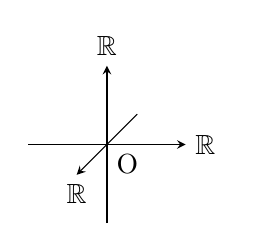
\begin{tikzpicture}

              \draw[-stealth](-1,0,0) -- (1,0,0) node[right]{$\mathbb{R}$};
              
              \draw[-stealth](0,-1,0) -- (0,1,0) node[above]{$\mathbb{R}$};
              
              \draw[-stealth](0,0,-1) -- (0,0,1) node[below]{$\mathbb{R}$};
              
              \draw (0,0,0) node[below right]{O};
            
            \end{tikzpicture}
          \end{figurehere}

          これを用いれば直積の交換法則が不成立な理由も次のように考えて直観的に理解できる。\par

          \subsubsection{幾何的に直積の交換法則が不成立であることを確認してみる}
            ある点$\ds (a, b)$を考えてみよう。(ただし$\ds a \ne b$とする。)\par
            もちろん$\ds a \ne b$であるから$\ds (a, b) \ne (b, a)$である。\par
            なぜなら順序対が反転したことで幾何的に異なる量へ変化したためである。

            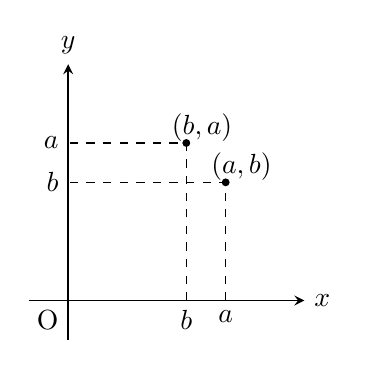
\begin{tikzpicture}
            
              \coordinate[label=below  left:O] (O) at (0,0); %原点O
              \coordinate (XS) at (-0.5,0); %x軸最小
              \coordinate (XL) at (3,0); %x軸最大
              \coordinate (YS) at (0,-0.5); %y軸最小
              \coordinate (YL) at (0,3); %y軸最大
              \draw[semithick,->,>=stealth] (XS)--(XL) node[right] {$x$}; %x軸
              \draw[semithick,->,>=stealth] (YS)--(YL) node[above] {$y$}; %y軸
              
              % (a, b)
              \coordinate (P1) at (2,1.5); %右頂点
              \fill (P1) circle (0.05); %点の塗りつぶし
              \node (x) at (2.2, 1.7) {$\ds (a, b)$};%座標の可視化
              
              % (b, a)
              \coordinate (P2) at (1.5,2); %右頂点
              \fill (P2) circle (0.05); %点の塗りつぶし
              \node (x) at (1.7, 2.2) {$\ds (b, a)$};%座標の可視化
              
              \draw[dashed] ($(XS)!(P1)!(XL)$)node[below]{$\ds a$}--(P1)--($(YS)!(P1)!(YL)$)node[left]{$\ds b$};
              \draw[dashed] ($(XS)!(P2)!(XL)$)node[below]{$\ds b$}--(P2)--($(YS)!(P2)!(YL)$)node[left]{$\ds a$};
                %右頂点から各軸への垂線
  
            \end{tikzpicture}

            これは幾何的に順序対が異なるものであることを説明しており、直積の順序で順序対が変化することが異なる量へ変化していることの証明といえるだろう。

        \subsection{参考: ユークリッド空間}
          先ほど$\ds \mathbb{R}$の直積を積み立てることで$\ds 2, 3$次元空間を集合で表現することができた。
          ではここでこれの一般化をしてみよう。\par
          次のように$\ds N \in \mathbb{N}$個の直積を考えてみる。

          \begin{equation*}
            \begin{split}
              $\ds \mathbb{R}^N = \{ (x_1, x_2, \cdots , x_N) \mid x_1 \in \mathbb{R}, x_2 \in \mathbb{R}, \cdots , x_N \in \mathbb{R} \}$
            \end{split}
          \end{equation*}

          % \[
          %   \left(
          %     \begin{tabular}{l}
          %       または次のようにも表せる。\\
          %       \begin{equation*}
          %         \begin{split}
          %           $\ds \mathbb{R}^3 = \{ (x, y, z) \mid x \in \mathbb{R}, y \in \mathbb{R}, z \in \mathbb{R} \}$\\
          %         \end{split}
          %       \end{equation*}
          %     \end{tabular}
          %   \right)
          % \]
          
          ここに得られた集合$\ds \mathbb{R}^N$をユークリッド空間という。\par
          つまり任意の$\ds N \in \mathbb{N}$に対して呼ぶのでもちろん$\ds \mathbb{R}^2$の$\ds 2$次元平面や$\ds \mathbb{R}^3$の$\ds 3$次元空間もユークリッド空間である。
      
    \end{multicols}

  \newpage

  \section{写像}
    前節では集合論の概要を説明した。ついでここでは集合間を関係づける概念、写像についてみておこう。
    \begin{multicols}{2}

      \subsection{写像の定義}
        $\ds X, Y$を空でない集合とする。\par
        任意の$\ds x \in X$に対し、ある$\ds y \in Y$が一意に定まるとき、このような対応規則を「$\ds X$から$\ds Y$への写像」と呼ぶ。\par
        また$\ds X, Y$が数を要素とする集合の場合特に関数と呼ぶ。つまり$\ds 関数 \subset 写像$である。\par
        簡潔に表現すれば以下。

        \vspace{9pt}\\

        $\ds f:X \mapsto Y \defineProposition \forall_{x \in X} [\exists!_{y \in Y} [y = f(x)]]$

        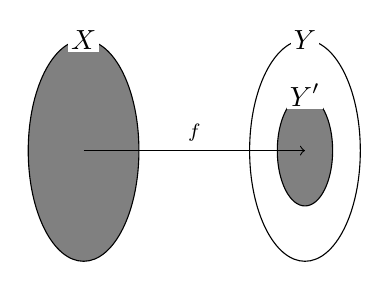
\begin{tikzpicture}[auto]
        
          %Xのベン図
          \fill[color=black!50!white, draw=black] (0,0) ellipse (20pt and 40pt);
          \node[set label,text=black] (X) at (0, 40pt) {$\ds X$};

          %Yのベン図
          \draw (80pt,0) ellipse (20pt and 40pt);
          \fill[color=black!50!white, draw=black] (80pt, 0) ellipse (10pt and 20pt); % black!50!white で黒と白50%
          \node[set label,text=black] (Y) at (80pt, 40pt) {$\ds Y$};
          \node[set label,text=black] (Y') at (80pt, 20pt) {$\ds Y'$};

          %写像f
          \draw[->] (0, 0) to node {$\scriptstyle f$} (80pt, 0);

        \end{tikzpicture}

      \subsection{定義域・値域}
        $\ds f:X \mapsto Y$において\par
        \begin{cases}
          $\ds X$を$\ds f$の定義域\\
          $\ds Y'(\subset Y)$を$\ds f$の値域\\
        \end{cases}
        という。\par

        値域$\ds R_f$の具体的な定義は以下。
      
        \vspace{9pt}\\

        $\ds R_f \defineProposition \{y \in Y \mid \exists_x [x \in X \wedge y=f(x)]\}$

        % \footnote{
        %   $\ds \exists_x [x \in X \wedge y=f(x)]$は自由変項$\ds y$が残るため$\ds y$の条件と言える。
        % }

      \subsection{単射(行先がかぶらない写像)}
        写像にはいくつか特性が存在する。その特性の一つを有する写像が単射と呼ばれるものである。\par
        $\ds f:X \mapsto Y$が単射であるとは、任意の$x,x'\in X$に対して「$\ds x \ne x' \Longrightarrow f(x) \ne f(x')$」が成立することである。\par
        つまり簡潔に表せば以下。

        \begin{equation}
          \begin{split}\notag
            $\ds f:X \mapsto Yが単射$     & $\defineProposition      \forall_{x,x'\in X} [x \ne x' \Longrightarrow f(x) \ne f(x')]$\\
                                          & $\ds \Longleftrightarrow  \forall_{x,x'\in X} [f(x) = f(x') \Longrightarrow x = x']$\\
          \end{split}
        \end{equation}

        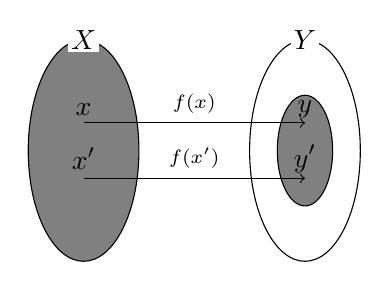
\begin{tikzpicture}[auto]
        
          %Xのベン図
          \fill[color=black!50!white, draw=black] (0,0) ellipse (20pt and 40pt);
          \node[set label, text=black] (X) at (0, 40pt) {$\ds X$};

          %Yのベン図
          \draw (80pt,0) ellipse (20pt and 40pt);
          \fill[color=black!50!white, draw=black] (80pt, 0) ellipse (10pt and 20pt); % black!50!white で黒と白50%
          \node[set label, text=black] (Y) at (80pt, 40pt) {$\ds Y$};

          %x->y
          \node (x) at (0, 15pt) {$\ds x$};
          \node (y) at (80pt, 15pt) {$\ds y$};
          \draw[->] (0, 10pt) to node {$\scriptstyle f(x)$} (80pt, 10pt);

          %x'->y'
          \node (x') at (0, -3pt) {$\ds x'$};
          \node (y') at (80pt, -3pt) {$\ds y'$};
          \draw[->] (0, -10pt) to node {$\scriptstyle f(x')$} (80pt, -10pt);

        \end{tikzpicture}

      \subsection{全射}
        写像の特使の一つを有するものを単射と言った。他にも全射と呼ばれるものもある。\par
        $\ds f:X \mapsto Y$が全射であるとは、任意の$y \in Y$に対して、ある$\ds x \in X$が存在し$\ds f(x)=y$となることである。\par
        つまり簡潔に表せば以下。

        \begin{equation}
          \begin{split}\notag
            $\ds f:X \mapsto Yが全射$     & $\defineProposition      \forall_{y\in Y} [\exists_{x\in X} [f(x) = y]]$\\
          \end{split}
        \end{equation}

        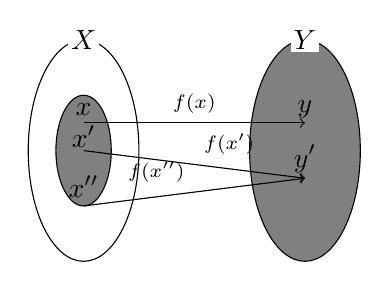
\begin{tikzpicture}[auto]
        
          %Xのベン図
          \draw (0,0) ellipse (20pt and 40pt);
          \fill[color=black!50!white, draw=black] (0, 0) ellipse (10pt and 20pt); % black!50!white で黒と白50%
          \node[set label, text=black] (X) at (0, 40pt) {$\ds X$};

          %Yのベン図
          \fill[color=black!50!white, draw=black] (80pt,0) ellipse (20pt and 40pt);
          \node[set label, text=black] (Y) at (80pt, 40pt) {$\ds Y$};

          %x->y
          \node (x) at (0, 15pt) {$\ds x$};
          \node (y) at (80pt, 15pt) {$\ds y$};

          %x'->y'
          \node (x') at (0, 5pt) {$\ds x'$};
          \node (y') at (80pt, -3pt) {$\ds y'$};

        %x''->y'
          \node (x'') at (0, -13pt) {$\ds x''$};

          \draw[->] (0, 10pt) to node {$\scriptstyle f(x)$} (80pt, 10pt);
          \draw[->] (0, 0) to node {$\scriptstyle f(x')$} (80pt, -10pt);
          \draw[->] (0, -20pt) to node {$\scriptstyle f(x'')$} (80pt, -10pt);

        \end{tikzpicture}

        \subsection{全単射(1対1対応、変換)}
        既に写像の特性を持つものを2つ紹介したが、これらの特性を同時に有する者ももちろん存在する。それを全単射といい、単射と全射それぞれの定義から成る合成命題で定義される。\par
        $\ds f:X \mapsto Y$が全単射であるとは、$\ds f$が単射かつ全射であるときをいう。\par
        また、定義域と値域が等しいことよりこの対応を1対1対応とも呼び、さらに互いの集合間をすべての要素が行き来できることより変換とも呼ぶ。(ただし変換に関しては必ずしも1対1対応でなくてもよい。)\par
        つまり簡潔に表せば以下。

        \begin{multline*}
          $\ds f:X \mapsto Yが全単射 \defineProposition \forall_{x,x'\in X} [f(x) = f(x') \Longrightarrow x = x']$\\
                                                        $\ds \wedge \forall_{y\in Y} [\exists_{x\in X} [f(x) = y]]$
        \end{multline*}

        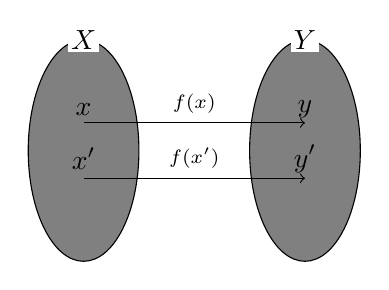
\begin{tikzpicture}[auto]
        
          %Xのベン図
          \fill[color=black!50!white, draw=black] (0,0) ellipse (20pt and 40pt);
          \node[set label, text=black] (X) at (0, 40pt) {$\ds X$};

          %Yのベン図
          \fill[color=black!50!white, draw=black] (80pt,0) ellipse (20pt and 40pt);
          \node[set label, text=black] (Y) at (80pt, 40pt) {$\ds Y$};

          %x->y
          \node (x) at (0, 15pt) {$\ds x$};
          \node (y) at (80pt, 15pt) {$\ds y$};
          \draw[->] (0, 10pt) to node {$\scriptstyle f(x)$} (80pt, 10pt);

          %x'->y'
          \node (x') at (0, -3pt) {$\ds x'$};
          \node (y') at (80pt, -3pt) {$\ds y'$};
          \draw[->] (0, -10pt) to node {$\scriptstyle f(x')$} (80pt, -10pt);

        \end{tikzpicture}

    \end{multicols}

\end{document}
